%!TEX TS-program = xelatex
%!TEX encoding = UTF-8 Unicode

\documentclass[12pt]{article}
\usepackage{geometry}                % See geometry.pdf to learn the layout options. There are lots.
\geometry{a4paper,top=2cm}
\usepackage[parfill]{parskip}    % Activate to begin paragraphs with an empty line rather than an indent
\usepackage{graphicx}
\usepackage{amsmath}
\usepackage{amssymb}
\usepackage{mathtools}
\usepackage{physics}
\newcommand{\be}{\begin{equation}}
\newcommand{\ee}{\end{equation}}
\usepackage[thicklines]{cancel}
\usepackage[colorlinks=true,citecolor=blue,linkcolor=blue,urlcolor=blue]{hyperref}
\usepackage{booktabs}
\usepackage{csquotes}
\usepackage{qcircuit}
\usepackage{circledsteps}
\usepackage{nicefrac}
\usepackage{fontspec,xltxtra,xunicode}
\usepackage{xcolor}
\usepackage{simplewick}
\defaultfontfeatures{Mapping=tex-text}

\newcommand{\polv}{\ensuremath{\updownarrow}}
\newcommand{\polh}{\ensuremath{\leftrightarrow}}
\newcommand{\poldr}{\rotatebox[origin=c]{45}{\ensuremath{\leftrightarrow}}}
\newcommand{\poldl}{\rotatebox[origin=c]{-45}{\ensuremath{\leftrightarrow}}}
\newcommand{\bigzero}{\mbox{\normalfont\Large\bfseries 0}}
\newcommand{\vecrp}{\ensuremath{\vec{r}^{\,\prime}}}
\newcommand{\vecnr}{\ensuremath{\vec{\nabla}_{\!r}}}

\title{Advanced Quantum Mechanics\\Class 06}
%\author{The Author}
\date{March 30, 2023}                                           % Activate to display a given date or no date

\setcounter{section}{2}
%\setcounter{subsection}{2}
%\setcounter{equation}{22}

\begin{document}
\maketitle

%%% 1 OK

\section{Entangled states and mixed states}

So far, single-particle states; many-particle states
richer configurations: \emph{entangled states}.
Even when particles are far apart (noninteracting),
they are correlated, and correlations cannot be
described classically.

\subsection{Tensor product of vector spaces}

\emph{Aim:} construct space of states of two physical systems.
\emph{First}, assume they are independent (noninteracting)
$H_1^N$ (dim $N$), $H_2^M$ (dim $M$): spaces of states of systems 1 and 2.
Since they are \emph{independent}, the state is defined by
specifying $\ket{\varphi} \in H_1^N$, $\ket{\chi} \in H_2^M$.
$\{
\ket{\varphi}, \ket{\chi}
\}$ -- assumed to be a vector belonging to
a vector space of dim $N \times M$ --
tensor product of $H_1$ and $H_2$
\be
H = H_1 \otimes H_2
\ee
More precise definition shortly ahead.

%%% 2 OK

\be
\left.
\begin{aligned}
\{\ket{n}\}: \text{ orthonormal basis of } H_1^N\\
\\
\{\ket{m}\}: \text{ orthonormal basis of } H_2^M
\end{aligned}
\right\}
\begin{aligned}
|\varphi\rangle&=\sum_{n=1}^{N} c_{n}|n\rangle\\
|\chi   \rangle&=\sum_{m=1}^{M} d_{m}|m\rangle\\
\end{aligned}
\ee
Space $H_1^N \otimes H_2^M$ \emph{defined} as a space of dim $N \times M$ where
\begin{enumerate}
\item $\{\ket{n}, \ket{m}\} \equiv \ket{n\otimes m}$ or $\ket{n}\otimes \ket{m}$ form an
orthonormal basis:
\be
\left\langle n^{\prime} \otimes m^{\prime} | n \otimes m\right\rangle=
\delta_{n n^{\prime}}
\delta_{m m^{\prime}}
\ee
%
\item and the tensor product of $\ket{\varphi}$ and $\ket{\chi} \equiv \ket{\varphi \otimes \chi}$
or $\ket{\varphi} \otimes \ket{\chi}$ is a vector with components $c_n d_m$
in the basis $\ket{n \otimes m}$:
\be
|\varphi\rangle \otimes|x\rangle=\sum_{n=1}^{N} \sum_{m=1}^{M} c_{n} d_{m}|n \otimes m\rangle
\ee
\end{enumerate}

\emph{Tensor product is linear:}

\be
\begin{aligned}
\left.\left.|\varphi \otimes( \chi_{1}+\lambda \chi_{2}\right)\right\rangle &=\left|\varphi \otimes \chi_{1}+\lambda \varphi \otimes \chi_{2}\right\rangle \\ &=\left|\varphi \otimes \chi_{1}\right\rangle+\left|\lambda \varphi \otimes \chi_{2}\right\rangle \\ &\left.=| \varphi \otimes \chi_{1}\right)+\lambda\left|\varphi \otimes \chi_{2}\right\rangle 
\end{aligned}
\ee

\be
\begin{aligned}
\left|\left(\varphi_{1}+\lambda \varphi_{2}\right) \otimes \chi\right\rangle &=\left|\varphi_{1} \otimes \chi+\lambda \varphi_{2} \otimes \chi\right\rangle \\ &=\left|\varphi_{1} \otimes \chi\right\rangle+\left|\lambda \varphi_{2} \otimes \chi\right\rangle \\ &=\left|\varphi_{1} \otimes \chi\right\rangle+\lambda\left|\varphi_{2} \otimes \chi\right\rangle
\end{aligned}
\ee

\emph{Tensor product is independent of basis:}

\be
|i\rangle=\sum_{n} R_{i n}|n\rangle, \quad|j\rangle=\sum_{m} S_{j m}|m\rangle
\ee
%%% 3 OK
$R,S$ unitary matrices. Tensor product in basis
$\ket{i},\ket{j}$ is given by:
\be
\begin{aligned}
|\varphi \otimes \chi\rangle 
&=\sum_{i, j} \bar{c}_{i} \bar{d}_{j}|i \otimes j\rangle=\sum_{i, j} \bar{c}_{i} \bar{d}_{j}|i\rangle \otimes|j\rangle\\
&=\sum_{i j} \bar{c}_{j} \bar{d}_{j} \sum_{n, m} R_{i n} S_{j m} |n\rangle \otimes|m\rangle\\
&=\sum_{n, m}
\underbrace{\left(\sum_{i} \bar{c}_{i} R_{i n}\right)}%
_{c_n}
\underbrace{\left(\sum_{j} \bar{d}_{j} R_{j m}\right)}%
_{d_n}
|n \otimes m\rangle\\
&=\sum_{n, m} c_{n} d_{n}|n \otimes m\rangle=|\varphi \otimes \chi\rangle
\end{aligned}
\ee
\emph{Now,} assume systems are \emph{not} independent.

\emph{Postulate V:} the space of states of two interacting systems
is $H_1^N \otimes H_2^M$ [identical particles: $N=M$,
only subspaces of $H_1^N \otimes H_2^M$ is physical].

The most general state vector in $H_{1}^{N} \otimes H_{2}^{M}$ is of the form:
\be
|\Phi\rangle=\sum_{n, m} b_{n m}|n \otimes m\rangle
\ee
where in general, the coefficient $b_{n m}$ is \emph{not} factorizable, i.e.
\be
b_{n m} \neq c_{n} d_{m}
\ee
%%% 4 OK
A state vector that cannot be written in the form
of a tensor product is named \emph{entangled state}.

$\hat{A},\hat{B}$: linear operators, $\hat{A}$ in $H_1^N$ and $\hat{B}$ in $H_2^M$. 
$\hat{C} = \hat{A} \otimes \hat{B}$ is the tensor product of $\hat{A}$ and $\hat{B}$.
Acts on $|\varphi \otimes \chi\rangle$ by definition as
\be
\begin{gathered}
\hat{C}|\varphi \otimes \chi\rangle=
|\hat{C}(\varphi \otimes \chi)\rangle=
|(\hat{A} \otimes \hat{B})(\varphi \otimes \chi)\rangle\\
=|\hat{A} \varphi \otimes \hat{B} \chi\rangle
\end{gathered}
\ee
Matrix elements of $\hat{C}$ in $\{|n \otimes m\rangle\}$ basis of $H_{1}^{N} \otimes H_{2}^{M}$:
\be
\left\langle n^{\prime} \otimes m^{\prime}|\hat{C}| n \otimes m\right\rangle=A_{n^{\prime}n} B_{m^{\prime}m}
\ee
%%% setcounter
\setcounter{equation}{11}
For a $\hat{C}$ in $H_{1}^{N} \otimes H_{2}^{M}$ which \emph{is not} of the form $\hat{A}\otimes\hat{B}$,
its elements in $\{(n \times m)\}$ are denoted by
\be
\left\langle n^{\prime} \otimes m^{\prime}|\hat{C}| n \otimes m\right\rangle=C_
{n^{\prime}n;m^{\prime}m}
\ee

\emph{Special cases:} 
\begin{enumerate}
\item $\hat{A} = I_1$ (identity in $H_{1}^{N}$)
\be
\begin{gathered}
\hat{A} \otimes \hat{B}|\varphi \otimes \chi\rangle = \left(I_{1} \otimes \hat{B}\right)|\varphi \otimes \chi\rangle = |\varphi \otimes \hat{B} \chi\rangle \\ 
\left\langle n^{\prime} \otimes m^{\prime}|\hat{A} \otimes \hat{B}| n \otimes m\right\rangle=\left\langle n^{\prime}|I| n\right\rangle\left\langle m^{\prime}|\hat{B}| m\right\rangle\\
= \delta_{n^{\prime}n} B_{m^{\prime}m}
\end{gathered}
\ee
%%% 5 OK
\item $\hat{B} = I_2$ (identity in $H_{2}^{M}$)
\be
\hat{A} \otimes \hat{B}|\varphi \otimes x\rangle = |\hat{A} \varphi \otimes \hat{B} \chi\rangle\\
\left\langle n^{\prime} \otimes m^{\prime}|\hat{A} \otimes \hat{B}| n \otimes m\right\rangle = 
A_{n^{\prime}n} \delta_{m^{\prime}m}
\ee 
\end{enumerate}

If $\hat{A}|\varphi\rangle=a|\varphi\rangle \Rightarrow|\varphi \otimes x\rangle$ is eigenvector
of $\hat{A}\otimes I_2$ with eigenvalue $a$:
\be
\left(\hat{A} \otimes I_{2}\right)\left|\varphi \otimes \chi\right\rangle=|\hat{A} \varphi \otimes \chi\rangle=a|\varphi \otimes \chi\rangle
\ee
and omitting $\otimes$
\be
\hat{A}|\varphi x\rangle=a|\varphi x\rangle
\ee
Since the notation $\otimes$ is cumbersome, we will
not use it when there is no danger of
confusion.

\subsection{System of two spins 1/2}

$H_1$ and $H_2$ are of dim. 2 $\Rightarrow$ $H_1$ and $H_2$ has dim. 4.
Bases of $H_1$ and $H_2$: eigenstates $\ket{\varepsilon_1}$ and $\ket{\varepsilon_2}$,
with $\varepsilon_i = \pm 1$, of the operators $\hat{S}_{1Z}$ and $\hat{S}_{2Z}$:
\begin{enumerate}
\item
\be
\begin{aligned}
\hat{S}_{1Z} \ket{\varepsilon_1} &= \frac{\hbar}{2} \varepsilon_1 \ket{\varepsilon_1}\\
\hat{S}_{2Z} \ket{\varepsilon_2} &= \frac{\hbar}{2} \varepsilon_2 \ket{\varepsilon_2}
\end{aligned}
\ee
therefore
\be
\begin{aligned}
(\hat{S}_{1Z} \otimes I_2) \ket{\varepsilon_1 \otimes \varepsilon_2} &= \hat{S}_{1Z} \ket{\varepsilon_1 \varepsilon_2}\\
&=\hbar/2 \varepsilon_1 \ket{\varepsilon_1 \varepsilon_2}
\end{aligned}
\ee
%%% 6 OK
\be
\begin{aligned}
(I_1 \otimes \hat{S}_{2Z}) \ket{\varepsilon_1 \otimes \varepsilon_2} &= \hat{S}_{2Z} \ket{\varepsilon_1 \varepsilon_2}\\
&=\hbar/2 \varepsilon_2 \ket{\varepsilon_1 \varepsilon_2}
\end{aligned}
\ee
%
\item
\be
\hat{S}_{1Z}\hat{S}_{2Z} \ket{\varepsilon_1 \varepsilon_2} = (\hbar/2)^2 \varepsilon_1 \varepsilon_2 \ket{\varepsilon_1 \varepsilon_2}
\ee
\end{enumerate}

Let $\ket{\chi_1} \in H_1$ and $\ket{\chi_2} \in H_2$: 
\be
\begin{aligned}
\left|\chi_{1}\right\rangle&=\lambda_{1}\left|+_{1}\right\rangle+\mu_{1}\left|-_{1}\right\rangle,\left|\lambda_{1}\right|^{2}+\left|\mu_{1}\right|^{2}=1\\
\left|\chi_{2}\right\rangle&=\lambda_{2}\left|+_{2}\right\rangle+\mu_{2}\left|-_{2}\right\rangle,\left|\lambda_{2}\right|^{2}+\left|\mu_{2}\right|^{2}=1
\end{aligned}
\ee
So the tensor product 
$\ket{\chi_1} \otimes \ket{\chi_2}$ = $\ket{\chi_1\otimes\chi_2}$ = $\ket{\chi_1\chi_2}$ 
is a sum of products of the form
$\ket{+_1} \otimes \ket{+_2}$ = $\ket{+_1\otimes+_2}$ = $\ket{+_1+_2}$,
$\ket{+_1} \otimes \ket{-_2}$ = $\ket{+_1\otimes-_2}$ = $\ket{+_1-_2}$,
\ldots:
\be
\ket{\chi_1\chi_2} = \lambda_1\lambda_2 \ket{++} + \lambda_1\mu_2 \ket{+-} +  \mu_1\lambda_2 \ket{-+} +  \mu_1\mu_2 \ket{--}
\ee
An arbitrary vector $\ket{\Psi}$ in $H = H_1 \otimes H_2$ in the $\{\varepsilon_1\varepsilon_2\}$ basis is given by:
\be
\ket{\Psi} = \alpha \ket{++} + \beta \ket{+-} +  \gamma \ket{-+} +  \delta \ket{--}
\ee
and cannot in general be written as a product of a $\ket{\chi_1} \in H_1$ and $\ket{\chi_2} \in H_2$; for this to be possible:
\be
\alpha\delta = \beta\gamma
\label{eq:g24}
\ee
%%% 7 OK
When Eq.~\eqref{eq:g24} is not satisfied $\rightarrow$ $\ket{\Psi}$ represents a two-spin entangled state.

\emph{Special examples:} of entangled state
\be
\ket{\Phi}_{\pm} = \frac{1}{\sqrt{2}}
\left(\ket{+-} \pm \ket{-+}\right)
\ee
where $\alpha = 0 = \delta$, $\beta = 1 = \pm \gamma$ $\Rightarrow 0 \neq \pm 1$.
It can be shown (\emph{Exercise}) that $\ket{\Phi}_-$ is invariant under rotations about an
arbitrary direction $\hat{n} = (\theta, \phi)$. $\ket{\Phi}_+$ is not!

\subsection{State operator}

Also known as density operator, density matrix.

Let $\ket{\Phi} \in H = H_1 \otimes H_2$. If $\ket{\Phi}$ is a tensor
product $\ket{\varphi_1 \otimes \varphi_2}$ $\rightarrow$ the state vector of particle 1
is $\ket{\varphi_1}$.
\emph{BUT}, if $\ket{\Phi}$ is an entangled state, i.e.
it \emph{cannot} be written as a product of a vector
in $H_1$ and another in $H_2$, one \emph{cannot}
associate a state vector to particle 1 (or 2).
This illustrates the fact that not always a state
vector can be assigned to a quantum system.
%%% 8 OK
One needs to generalize the description.

\emph{Pure state:} when a quantum system can be
described by a vector in a Hilbert space
-- complete information about the
system is available.

\emph{Mixture} (mixed state): when information is incomplete
$\Rightarrow$ system is described by a state operator
(statistical, kind of generalization of the projection operator).

For a pure state:
\be
\begin{aligned}
\langle\hat{A}\rangle
&=\langle\varphi|\hat{A}| \varphi\rangle=\sum_{n, m}\langle\varphi | n\rangle\langle n|\hat{A}| m\rangle\langle m | \varphi\rangle\\
&=\sum_{n, m}\langle m 
\underbrace{| \varphi\rangle\langle\varphi |}%
_{\hat{P}_\varphi}
n\rangle\langle n|\hat{A}| m\rangle\\
&=\sum_{m}\langle m |\hat{P}_{\varphi}
\underbrace{\left(\sum_{n}|n\rangle\langle n|\right)}%
_{1}
\hat{A}| m \rangle\\
&=\sum_m \bra{m}\hat{P}_\varphi\hat{A}\ket{m} = \operatorname{Tr}(\hat{P}_\varphi\hat{A})
\end{aligned}
\ee
Generalization when system is
in a mixture of states $\ket{\varphi_\alpha}$ .

%%% 9 OK
\[
\begin{aligned}
\langle\hat{A}\rangle 
&=\sum_{\alpha} p_{\alpha}\left\langle\varphi_{\alpha}|\hat{A}| \varphi_{\alpha}\right\rangle=\sum_{\alpha} p_{\alpha} \operatorname{Tr}\left(\hat{P}_{\varphi_{\alpha}} \hat{A}\right) \\ 
&=\sum_{\alpha} \operatorname{Tr}\left(p_{\alpha} \hat{P}_{\alpha} \hat{A}\right)\\
&=\operatorname{Tr}\left[
\underbrace{\left(\sum_{\alpha} p_{\alpha} \hat{P}_{\alpha}\right)}%
_{\hat{\rho}} 
\hat{A}\right]
\end{aligned}
\]
\be
\hat{\rho} \equiv \sum_\alpha p_\alpha \hat{P}_\alpha =
\sum_\alpha p_\alpha \op{\varphi_\alpha}{\varphi_\alpha}
\ee
where $p_\alpha$ is the probability in $\ket{\varphi_\alpha}$, fixed by the problem at hand.
For a pure state, $\rho_\alpha = \ket{\varphi}\bra{\varphi} = \hat{P}_\varphi.$

\emph{Properties:} (exercises)
\begin{enumerate}
\item \[\hat{\rho} = \hat{\rho}^\dagger\]
\item \be\operatorname{Tr}\hat{\rho} = 1\ee
\item $\hat{\rho}$ is positive operator: $\bra{\varphi}\hat{\rho}\ket{\varphi} \geq 0, \forall \ket{\varphi}$. This means that all of its eigenvalues are positive, see Exercise 2.4.10.
\item Pure state iff $\hat{\rho}^2 = \hat{\rho}$
\end{enumerate}

\subsection{State operator for a two-level system}

The standard example is a spin-1/2 system, Hilbert space of dim. 2.
We will use this to define notation and nomenclature.

Basis vector of the space of states: $\{\ket{+},\ket{-}\}$

$\hat{\rho}$ $\to$ matrix $\rho$: $2\times2$, Hermitian, trace 1, positive.
Its most general form is:
%%% 10 OK
\be
\rho = 
\begin{pmatrix}
a & c\\
c^* & (1-a)
\end{pmatrix}
\label{eq:g29}
\ee
with $a$ real and $c$ complex.
$\lambda_+,\lambda_-$: eigenvalues.
\be
\begin{gathered}
\text{Unit trace: }\lambda_+ + \lambda_- = 1\\
\text{Positive: }\lambda_+ \geq 0, \lambda_- \geq 0
\end{gathered}
\ee

Eigenvalues:
\[
\begin{gathered}
(a-\lambda)(1-a-\lambda)-|c|^{2}=0\\
(\alpha-\lambda)[(a+\lambda)-1]+|c|^{2}=0\\
a^{2}-\lambda^{2}-a+\lambda+|c|^{2}=0 \,\therefore\,
\lambda^{2}-\lambda+\left[a(1-a)-|c|^{2}\right]=0
\end{gathered}
\]
hence
\be
\begin{aligned}
\lambda_{\pm}
&=\frac{1}{2}\left[1 \pm \sqrt{1-4\left[a(1-a)-|c|^{2}\right]}\right]\\
&=\frac{1}{2} \pm \sqrt{\frac{1}{4}-\left[a(1-a)-|c|^{2}\right]}
\end{aligned}
\ee
\[
\begin{gathered}
\lambda_\pm \text{ real: }a(1-a)-|c|^{2} \leqslant 1 / 4\\
\lambda_+,\lambda_->0 \Rightarrow \det \rho>0: a(1-a)-|c|^{2} \geqslant 0
\end{gathered}
\]
\be
\boxed{
0 \leqslant a(1-a)-|c|^{2} \leqslant 1 / 4
}
\label{eq:g32}
\ee

For a pure state: $\ket{\psi}$, $\rho_\psi = \ket{\psi}\bra{\psi} = \hat{\rho}_\psi$
\be
|\psi\rangle=\lambda|+\rangle+\mu|-\rangle, \quad|\lambda|^{2}+|\mu|^{2}=1
\ee
%%% 11 OK
\be
\begin{aligned}
\hat{p}
&=\left(\lambda\ket{+}+\mu\ket{-}\right)
  \left(\lambda^{*}\bra{+}+\mu^{*}\bra{-}\right)\\
&=|\lambda|^2\ket{+}\bra{+}+
 \lambda\mu^*\ket{+}\bra{-}+
 \mu\lambda^*\ket{-}\bra{+}+
|\mu|^2      \ket{-}\bra{-}
\end{aligned}
\ee
therefore
\be
\rho_\psi = 
\begin{pmatrix}
\rho_{++} & \rho_{+-} \\ 
\rho_{-+} & \rho_{--}
\end{pmatrix}
=
\begin{pmatrix}
|\lambda|^2 & \lambda\mu^*\\
\mu\lambda^* & |\mu|^2 
\end{pmatrix}
\ee
and
\[
a=|\lambda|^{2}, c=\lambda \mu^{*}, \det \rho_{\psi}=|\lambda|^{2}|\mu|^{2}-\lambda \mu^{*} \mu \lambda^{*}=0
\]
So, for a pure state we see that:
\be
\boxed{\det \rho = 0} \Rightarrow a(1-a) - |c|^2 = 0 
\ee

Convenient to decompose $\rho$ as given in Eq.~\eqref{eq:g29} in
terms of Pauli matrices.
Parameterise $a$ and $c$ by three real numbers $b_x$, $b_y$, $b_z$:
%%% setcounter
\setcounter{equation}{35}
\be
\begin{aligned}
a&=1 / 2\left(1+b_{z}\right) \rightarrow 1-a=1 / 2\left(1-b_{z}\right) \\ 
c&=1 / 2\left(b_{x}-i b_{y}\right)
\end{aligned}
\ee
hence
\be
\rho=1 / 2
\begin{pmatrix}
1+b_{z} & b_{x}-i b_y \\ 
b_{x}+i b_y & 1-b_{z}
\end{pmatrix}
= \frac{1}{2} (I + \vec{b}\cdot\vec{\sigma})
\ee
where $\vec{b}$ is the Bloch vector.

In Eq.~\eqref{eq:g32}: $0 \leqslant a(1-a)-|c|^{2} \leqslant 1 / 4$, so
$0 \leq 1 / 4\left(1+b_{z}\right)\left(1-b_{z}\right)-1 / 4\left(b_{x}^{2}+b_{y}^{2}\right)
= 1/4 (1 - |\vec{b}|^2) \leqslant 1/4$
\be
\boxed{
|\vec{b}|^2 \leqslant 1 
}
\ee

%%%% 12 OK

\emph{Pure state:} $\operatorname{det} \rho=0 \Rightarrow 1 / 4\left[1-b_{z}^{2}-\left(b_{x}^{2}+b_{y}^{2}\right)\right]=0$, therefore
\be
\boxed{
|\vec{b}|^2 = 1 
}
\ee

Physical interpretation of $\vec{b}$:
\be
\begin{aligned}
\langle\hat{S}_i\rangle &
= \Tr \hat{\rho} \hat{S}_i = \frac{1}{2} \hbar \Tr
\left[
 \frac{1}{2} (I + \vec{b}\cdot\vec{\sigma}) \sigma_i
\right]\\
&=\frac{1}{2} \hbar\left[\frac{1}{2} \underbrace{\Tr \sigma_{i}}_0
+\frac{1}{2} b_{j} \Tr \sigma_{j} \sigma_{i}
\right]%
\quad,\text{but } \sigma_{j} \sigma_{i} = 
\underbrace{\delta_{ji}}_{I} \,+ 
\underbrace{\epsilon_{ijk}\sigma_k}_{\text{trace is null}}\\
&=\frac{1}{2} \hbar \frac{1}{2} b_{i} \Tr I=\frac{1}{2} \hbar b_{i}
\end{aligned}
\ee
which means
\be
\boxed{
\langle\vec{S}\,\rangle = \frac{1}{2} \hbar \vec{b}
}
\ee
so
\[
\begin{gathered}
\vec{b} = 0: \text{ unpolarized system} \\
|\vec{b}| = 1: \text{ polarized system} \\
0 \leqslant |\vec{b}| \leqslant 1: \text{ partially polarized system}
\end{gathered}
\]

\emph{Bloch sphere:} sphere of unit radius, $\vec{b} = \overrightarrow{OP}$.
Let two other arbitrary unit vectors in that sphere $\hat{n}_1$, $\hat{n}_2$:
\be
\hat{n}_1 = \overrightarrow{OP_1}, \hat{n}_2 = \overrightarrow{OP_2}
\ee
Can always write $\vec{b}$ in terms of the two unitary vectors (\emph{Exercise}):
\be
\begin{aligned} 
\vec{b}&= \hat{n}_1 + \lambda(\hat{n}_2 - \hat{n}_1)\\
&= (1-\lambda) \hat{n}_1 + \lambda\hat{n}_2
\end{aligned}
\ee
All the vectors in the Bloch sphere represent pure states, $|\vec{b}| = 1$.
In contrast, all the vectors in the interior ball described by that sphere represent mixed states,
$|\vec{b}| \leqslant 1$ (more on that later).
\begin{center}
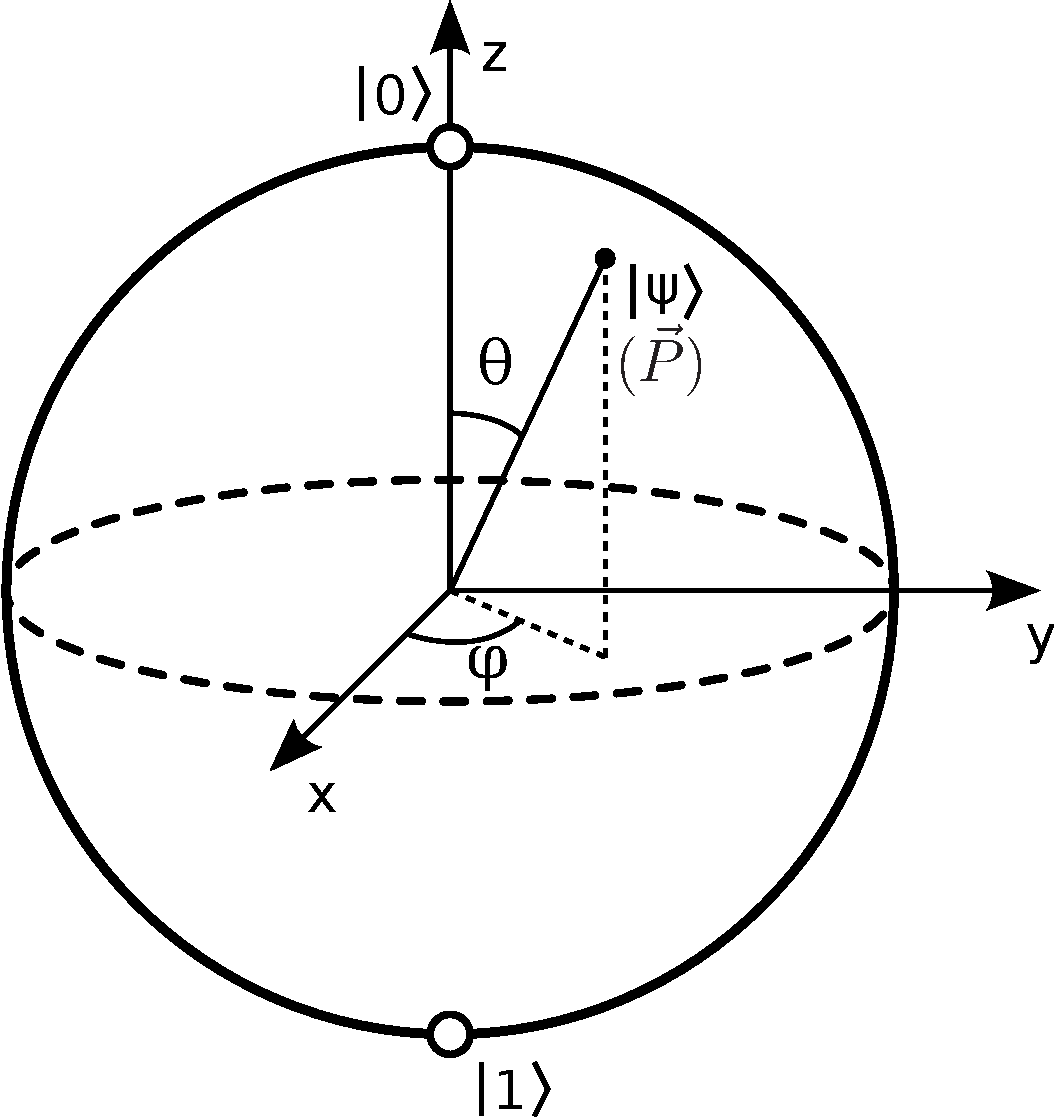
\includegraphics[width=0.5\textwidth]{Figures/Bloch_sphere.pdf}\\
\scriptsize{\texttt{By Smite-Meister - Own work, CC BY-SA 3.0, https://commons.wikimedia.org/w/index.php?curid=5829358}}
\end{center}

%%% 13 OK

In terms of $\hat{n}_1$ and $\hat{n}_2$, $\rho$ matrix can be written as:
\be
\begin{aligned} \rho = 1 / 2(1+\vec{b} \cdot \vec{\sigma}) 
&=1 / 2\left[1+(1-\lambda) \hat{n}_{1} \cdot \vec{\sigma}+\lambda \hat{n}_{2} \cdot \vec{\sigma}\right] \\ 
&=(1-\lambda) \frac{1}{2}\left(1+\hat{n}_{1} \cdot \vec{\sigma}\right)+\lambda \frac{1}{2}\left(1+\hat{n}_{2}\cdot \vec{\sigma}\right) \end{aligned}
\ee
$\frac{1}{2}(1+\hat{n}_{1}\cdot\vec{\sigma})$: pure state (polarized), since $\hat{n}_{1}$ is a unit vector.
%as two spin-1/2 systems with $S=0$, or $S=1$, or single-spin systems.
So, we can decompose an arbitrary density matrix $\rho$ in a sum of pure states.

$\rho$ describes a quantum state with \emph{statistical
mixture} with probabilities:
\be
p_{1}=1-\lambda \quad \text { and } \quad p_{2}=\lambda
\ee
Since there an infinite number of $\lambda$ values with
$0<\lambda<1$ giving same $\vec{b}$, there is an infinite
number of ways of preparing a quantum
state described by $\rho=\frac{1}{2}(1+\vec{b} \cdot \vec{\sigma})$.

Important to distinguish \emph{pure} and \emph{mixture} states.
Example: single-spin state, eigenstate of $\hat{S}_x$
\be
|\chi\rangle=\frac{1}{\sqrt{2}}[|+\rangle+|-\rangle]=|+, \hat{x}\rangle
\ee
\be
\rho=\frac{1}{2}
\begin{pmatrix}
1 & 1 \\ 1 & 1
\end{pmatrix}, \vec{b}=(1,0,0)
\ee
In a Stern-Gerlach experiment, when $\vec{B}=B\hat{z}$,
50\% prob. spin $\uparrow\,= \ket{+}$ and 50\% spin $\downarrow\,= \ket{-}$
%%% 14 OK
But when $\hat{B} = B\hat{x}$ $\to$ 100\% in state $\ket{\chi} = \ket{+,\hat{x}}$.

Now, for a state with $\vec{b} = 0$:
\be
\begin{aligned}
\rho 
&= \frac{1}{2}
\begin{pmatrix}
1 & 0\\0 & 1
\end{pmatrix}
=
\frac{1}{2}
\begin{pmatrix}
1 & 0\\0 & 0
\end{pmatrix}+
\frac{1}{2}
\begin{pmatrix}
0 & 0\\0 & 1
\end{pmatrix}\\
&=1/2\ket{+}\bra{+} + 1/2\ket{-}\bra{-}\\
&=1/2\times
\underbrace{1/2(1+\hat{z} \cdot \vec{\sigma})}%
_{\text{pure in }\hat{z}} + 
1/2\times
\underbrace{1/2(1+(-\hat{z}) \cdot \vec{\sigma})}%
_{\text{pure in }-\hat{z}}
\end{aligned}
\ee
so it is a statistical mixture of $\ket{+,\hat{z}}$ and $\ket{+,-\hat{z}} = \ket{-,\hat{z}}$ 
When $\vec{B} = B\hat{z}$ in Stern-Gerlach apparatus:
50\% $\uparrow(+\hat{z})$ and 50\% $\downarrow(-\hat{z})$
When $\vec{B} = B\hat{n}$, \emph{again}
50\% $(+\hat{n})$ and 50\% $(-\hat{n})$;
trivially if $\vec{b}=1 / 2 \hat{n}+1 / 2(-\hat{n})$
\be
1/2\times
\underbrace{1/2(1+\hat{n} \cdot \vec{\sigma})}%
_{\text{pure in }\hat{n}} + 
1/2\times
\underbrace{1/2(1+(-\hat{n}) \cdot \vec{\sigma})}%
_{\text{pure in }-\hat{n}}
\ee
\emph{Difference} between
$1/2
\begin{pmatrix}
1 & 1\\1 & 1
\end{pmatrix}
$ (polarized)
and 
$1/2
\begin{pmatrix}
1 & 0\\0 & 1
\end{pmatrix}
$ (unpolarized).
The former is a \emph{coherent} superposition $\ket{+}$, $\ket{-}$ with
well-defined phase for finding $\ket{+}$, $\ket{-}$.
The latter is an \emph{incoherent} mixture,
phase is lost.
\emph{Phase information} $\to$ in the \emph{off-diagonal} elements of $\rho$,
which are called coherences of the state vector.




















\end{document} 